% thiếu: 3.3, 3.2
% target: 15 pages
\mychapter{3}{CHAPTER 3. METHODS} \label{ch:chap3} \graphicspath{{./chapter3/image/}}

This chapter proposes a general pipeline for on-device vision applications and a method based on deep learning solving hair segmentation and clothing segmentation tasks. Aside from that, methods for overlaying a mask on a photograph are also demonstrated. \par
Concerning the pipeline for the Android application, I first list all use cases for the app and then do further analysis on them. With some intricate use cases having many classes involved, sequence diagrams are provided to illustrate how these classes work together. Such generic prototypes can be reused later, whenever camera application development is needed. \par
In terms of the deep learning model, every component of the proposed network will be explained in this chapter. The proposed method for optimizing the model and converting it to TFLite's supported format will also be presented. The practical performance and accuracy of the proposed method will be discussed in the next chapter.\par

\section{Use-Case Analysis and Design} \label{sec:usecase}

\subsection{Use Case}
This sector defines the functional requirements for the app. In summary, the app has \textbf{1 actor} and \textbf{10 use cases}. An actor models a type of role played by an entity that interacts with the app. The actor can be a human user or an external system. Meanwhile, a use case describes a sequence of interactions between actors and systems to accomplish a particular goal. Use cases are usually referred to as system functionalities that a system should perform in interaction with one or more external users (actors). In the case of the thesis, the actor is the users, and the system is the mobile application. The figure below is the proposed UML \cite{uml} use case diagram: \par

\begin{figure} [H]
    \centering
    \captionsetup{justification=centering}
    \includegraphics[width=1.0\textwidth]{chapter3/image/use-case.png}
    \caption{Use case diagram for the hair and clothes app}
    \label{fig:schnet_LiNet}
\end{figure}

With each use case, it is accompanied by a table describing it. In tables, the "Pre-condition" row is a list of conditions that must be met before the action of that use case. The "Post-condition" row is a list of conditions that must be reached after the action of that use case. The "Expected result" row lists acceptable results of that use case.

\begin{center} 
\begin{table} [H]
\caption{Hair camera use-case description} 
\begin{tabular}{p{0.35\linewidth} | p{0.6\linewidth}}
\hline
USER CASE            & UC-1 \\ \hline
Use case name        & Hair Camera   \\ \hline
Use case description & Real-time camera preview with hair \\ \hline
Pre-condition         &   User were in the app's main screen, selected the “Hair Camera” option. Request permissions must be accepted before camera starts \\ \hline
Post-condition        &   Camera preview is displayed in response to the hardware. Hair mask is overlayed directly on frames  \\ \hline
Basic flow           &   \begin{enumerate}
    \item User switches front to rear camera, and vice versa.
    \item User changes color of hair.
    \item User clicks the capture button.
\end{enumerate}   \\ \hline
Alternate flows      &   \begin{enumerate}
    \setcounter{enumi}{3}
    \item User clicks the back button
\end{enumerate}   \\ \hline
Expected result      &  \begin{enumerate}
    \item If permissions are not granted, ask for the permissions.
\end{enumerate}    \\ \hline
\end{tabular}
\end{table}
\end{center}


\begin{center}
\begin{table} [H]
\caption{Clothes camera use-case description} 
\begin{tabular}{p{0.35\linewidth} | p{0.6\linewidth}}
\hline
USER CASE            & UC-2 \\ \hline
Use case name        & Clothes Camera  \\ \hline
Use case description & Real-time camera preview with clothes recolored     \\ \hline
Pre-condition         &   User were in the app's main screen, selected the “Clothes Camera” option. Request permissions must be accepted before camera starts   \\ \hline
Post-condition        &   Camera preview is displayed in response to the hardware. Clothes mask is directly overlaied on frames   \\ \hline
Basic flow           &  \begin{enumerate}
  \item Users switch front to rear camera, and vice versa.
  \item Users change color for clothes.
  \item	Users click the capture button. 
\end{enumerate} \\ \hline
Alternate flows      &   \begin{enumerate}
    \setcounter{enumi}{3}
    \item User clicks the back button, returning to the main screen
\end{enumerate}   \\ \hline
Expected result      &  \begin{enumerate}
    \item If permissions are not granted, ask for the permissions
\end{enumerate}    \\ \hline
\end{tabular}
\end{table}
\end{center}


\begin{center}
\begin{table} [H]
\caption{Change lens use-case description} 
\begin{tabular}{p{0.35\linewidth} | p{0.6\linewidth}}
\hline
USER CASE            & UC-3 \\ \hline
Use case name        &  Change lens  \\ \hline
Use case description &   One button is responsible for switching between front and rear lens  \\ \hline
Pre-condition         &   Camera preview is displayed, but user want to the other camera instead   \\ \hline
Post-condition        &   Preferable camera lens is chosen. User is now ready for capture.   \\ \hline
Basic flow           &  \begin{enumerate}
  \item User clicks on lens switching button.
  \item	Preview camera displays image for the front camera if the rear camera is opening. 
  \item New mask is generated and replaces the old one.
\end{enumerate}    \\ \hline
Alternate flows      &   N/A   \\ \hline
Expected result      & \begin{enumerate}
    \item User is able to change between camera lenses multiple times.
\end{enumerate}     \\ \hline
\end{tabular}
\end{table}
\end{center}


\begin{center}
\begin{table} [H]
\caption{Capture use-case description} 
\begin{tabular}{p{0.35\linewidth} | p{0.6\linewidth}}
\hline
USER CASE            & UC-4 \\ \hline
Use case name        &  Capture \\ \hline
Use case description &  One button is responsible for capture from camera     \\\hline
Pre-condition         &   Camera preview is displayed, user switched to lens his/her want. Now, user want to capture the frame at that moment  \\ \hline
Post-condition        &   Frame is captured and ready for latter use  \\ \hline
Basic flow           &   \begin{enumerate}
    \item 	User clicks on capture button
\item Stop camera previewing
\item The frame at the moment is saved to memory
\item Show options to treat the captured frame
\end{enumerate}
\\ \hline
Alternate flows      & N/A     \\ \hline
Expected result      &  
\begin{enumerate}
    \item User is able to capture multiple times.
\end{enumerate}   \\ \hline
\end{tabular}
\end{table}
\end{center}


\begin{center}
\begin{table} [H]
\caption{Clothes segmentation use-case description} 
\begin{tabular}{p{0.35\linewidth} | p{0.6\linewidth}}
\hline
USER CASE            & UC-5 \\ \hline
Use case name        &  Clothes segmentation  \\ \hline
Use case description &  Clothes color in a chosen image is recolored    \\\hline
Pre-condition         &   User was in the app’s main screen, selected the “Clothes segmentation” option. Permission requests must be accepted before camera starts   \\ \hline
Post-condition        &   Input image is recolored and applied filter. User gets recolored image his/her want.   \\ \hline
Basic flow           &   \begin{enumerate}
    \item Choose an image from gallary
\item Choose color for clothes in image
\item Choose filter that is going to apply to the image
\item Save \& Share the new image
\end{enumerate}
   \\ \hline
Alternate flows      &    \begin{enumerate}
    \setcounter{enumi}{4}
    \item User clicks on Back button, return to the main screen
\end{enumerate}  \\ \hline
Expected result      &  \begin{enumerate}
    \item If user chooses unsupported file format, showing up this error
\item New image is saved and shared successfully
\end{enumerate}    \\ \hline
\end{tabular}
\end{table}
\end{center}

%finish

\begin{center}
\begin{table} [H]
\caption{Hair segmentation use-case description} 
\begin{tabular}{p{0.35\linewidth} | p{0.6\linewidth}}
\hline
USER CASE            & UC-6 \\ \hline
Use case name        &  Hair segmentation  \\ \hline
Use case description &  Hair color in a chosen image is recolored    \\\hline
Pre-condition         &   User was in the app’s main screen, selected the “Hair segmentation” option. Permission requests must be accepted before camera starts   \\ \hline
Post-condition        &   Input image is recolored and applied filter. User gets recolored image his/her want.   \\ \hline
Basic flow           &   \begin{enumerate}
    \item Choose an image from gallary
    \item Choose color for hair in image
    \item Choose filter that is going to apply to the image
    \item Save \& Share the new image
\end{enumerate}
   \\ \hline
Alternate flows      &    \begin{enumerate}
    \setcounter{enumi}{4}
    \item User clicks on Back button, return to the main screen
\end{enumerate}  \\ \hline
Expected result      &  \begin{enumerate}
    \item 	If user chooses unsupported file format, showing up this error
    \item 	New image is saved or shared successfully
\end{enumerate}    \\ \hline
\end{tabular}
\end{table}
\end{center}

\begin{center}
\begin{table} [H]
\caption{Hair color scanning use-case description} 
\begin{tabular}{p{0.35\linewidth} | p{0.6\linewidth}}
\hline
USER CASE            & UC-7 \\ \hline
Use case name        &  Hair color scanning  \\ \hline
Use case description &  Hair color on camera preview will continuously switch to all colors.    \\\hline
Pre-condition         &  User was in the app’s main screen, selected the “Hair color scanning” option. Permission requests must be accepted before camera starts    \\ \hline
Post-condition        &   User looked at his/her hair in different colors. User want to experience other user cases.   \\ \hline
Basic flow           &  \begin{enumerate}
    \item Camera opens, switching camera lens as user want
\item	Hair mask renders directly on camera preview

\end{enumerate}    \\ \hline
Alternate flows      &   \begin{enumerate}
    \setcounter{enumi}{2}
    \item User clicks on Back button, return to the main screen
\end{enumerate}   \\ \hline
Expected result      &  \begin{enumerate}
    \item Hair is recolored successfully
    \item User is able to change camera lens
\end{enumerate}    \\ \hline
\end{tabular}
\end{table}
\end{center}

\begin{center}
\begin{table} [H]
\caption{Select color use-case description} 
\begin{tabular}{p{0.35\linewidth} | p{0.6\linewidth}}
\hline
USER CASE            & UC-8 \\ \hline
Use case name        &  Select color  \\ \hline
Use case description &   User can select a color from color palette for mask. Hair or clothes would be changed to that color at once   \\\hline
Pre-condition         &   User are at preview camera with mask overlaid, but he/she want to change mask to a different color   \\ \hline
Post-condition        &   User chose his/her favorite color and come back to preview camera    \\ \hline
Basic flow           &  \begin{enumerate}
    \item 	User clicks on the color palette button
\item	A color palette shows up 
\item User clicks on the color his/her like
\item The color palette disappears, return to camera preview screen
\end{enumerate}    \\ \hline
Alternate flows      &   N/A   \\ \hline
Expected result      &  \begin{enumerate}
    \item 	If the chosen color is different with previous color, change mask’s color
\item If the color palette button is clicked in the second times, color palette disappears.
\end{enumerate}    \\ \hline
\end{tabular}
\end{table}
\end{center}

%finish

\begin{center} 
\begin{table} [H]
\caption{Apply filter use-case description} 
\begin{tabular}{p{0.35\linewidth} | p{0.6\linewidth}}
\hline
USER CASE            & UC-9 \\ \hline
Use case name        &  Apply filter  \\ \hline
Use case description &  Filters that is listed for user to edit image    \\\hline
Pre-condition         &   User after recoloring hair or clothes wants to edit the image more  \\ \hline
Post-condition        &   User finishes editting   \\ \hline
Basic flow           &  \begin{enumerate}
    \item Show filters available 
    \item User chooses an filter
    \item Preview image after apply filter
    \item User accept the filter
\end{enumerate}    \\ \hline
Alternate flows      &   N/A   \\ \hline
Expected result      &  \begin{enumerate}
    \item If user refuses to apply filter, image stayes the same
\end{enumerate}     \\ \hline
\end{tabular}
\end{table}
\end{center}

\begin{center} 
\begin{table} [H]
\caption{Save \& Share use-case description} 
\begin{tabular}{p{0.35\linewidth} | p{0.6\linewidth}}
\hline
USER CASE            & UC-10 \\ \hline
Use case name        &  Save \& Share  \\ \hline
Use case description &   Each image that is taken before, is opted to delete or save or share   \\\hline
Pre-condition         &   User clicked capture button   \\ \hline
Post-condition        &  Photograph is saved/shared and user want to take another    \\ \hline
Basic flow           &   \begin{enumerate}

    \item Show images that is captured before
    \item User clicks onto save button
    \item Image is saved into storage
    \item User clicks onto share button
    \item User choose where to share the image
    \item Return to preview camera screen
\end{enumerate}   \\ \hline
Alternate flows      &  \begin{enumerate}
    \setcounter{enumi}{6}
    \item User clicks back button, then return to preview camera screen
\end{enumerate}    \\ \hline
Expected result      &   
\begin{enumerate}
    \item An image can be both saved and shared
\end{enumerate}  \\ \hline
\end{tabular}
\end{table}
\end{center}

\subsection{Sequence Diagram}

In this phase, we are going to discuss diagrams showing the interactions between objects in the app, arranged
in a sequence. These following diagrams also show a series of messages exchanged by objects that perform a specific task or action. Clothes Camera and Hair Segmentation use cases are chosen to elaborate with sequence diagrams, as these use cases are representative and substantial in the app.  

\begin{figure}[H]
    \centering
    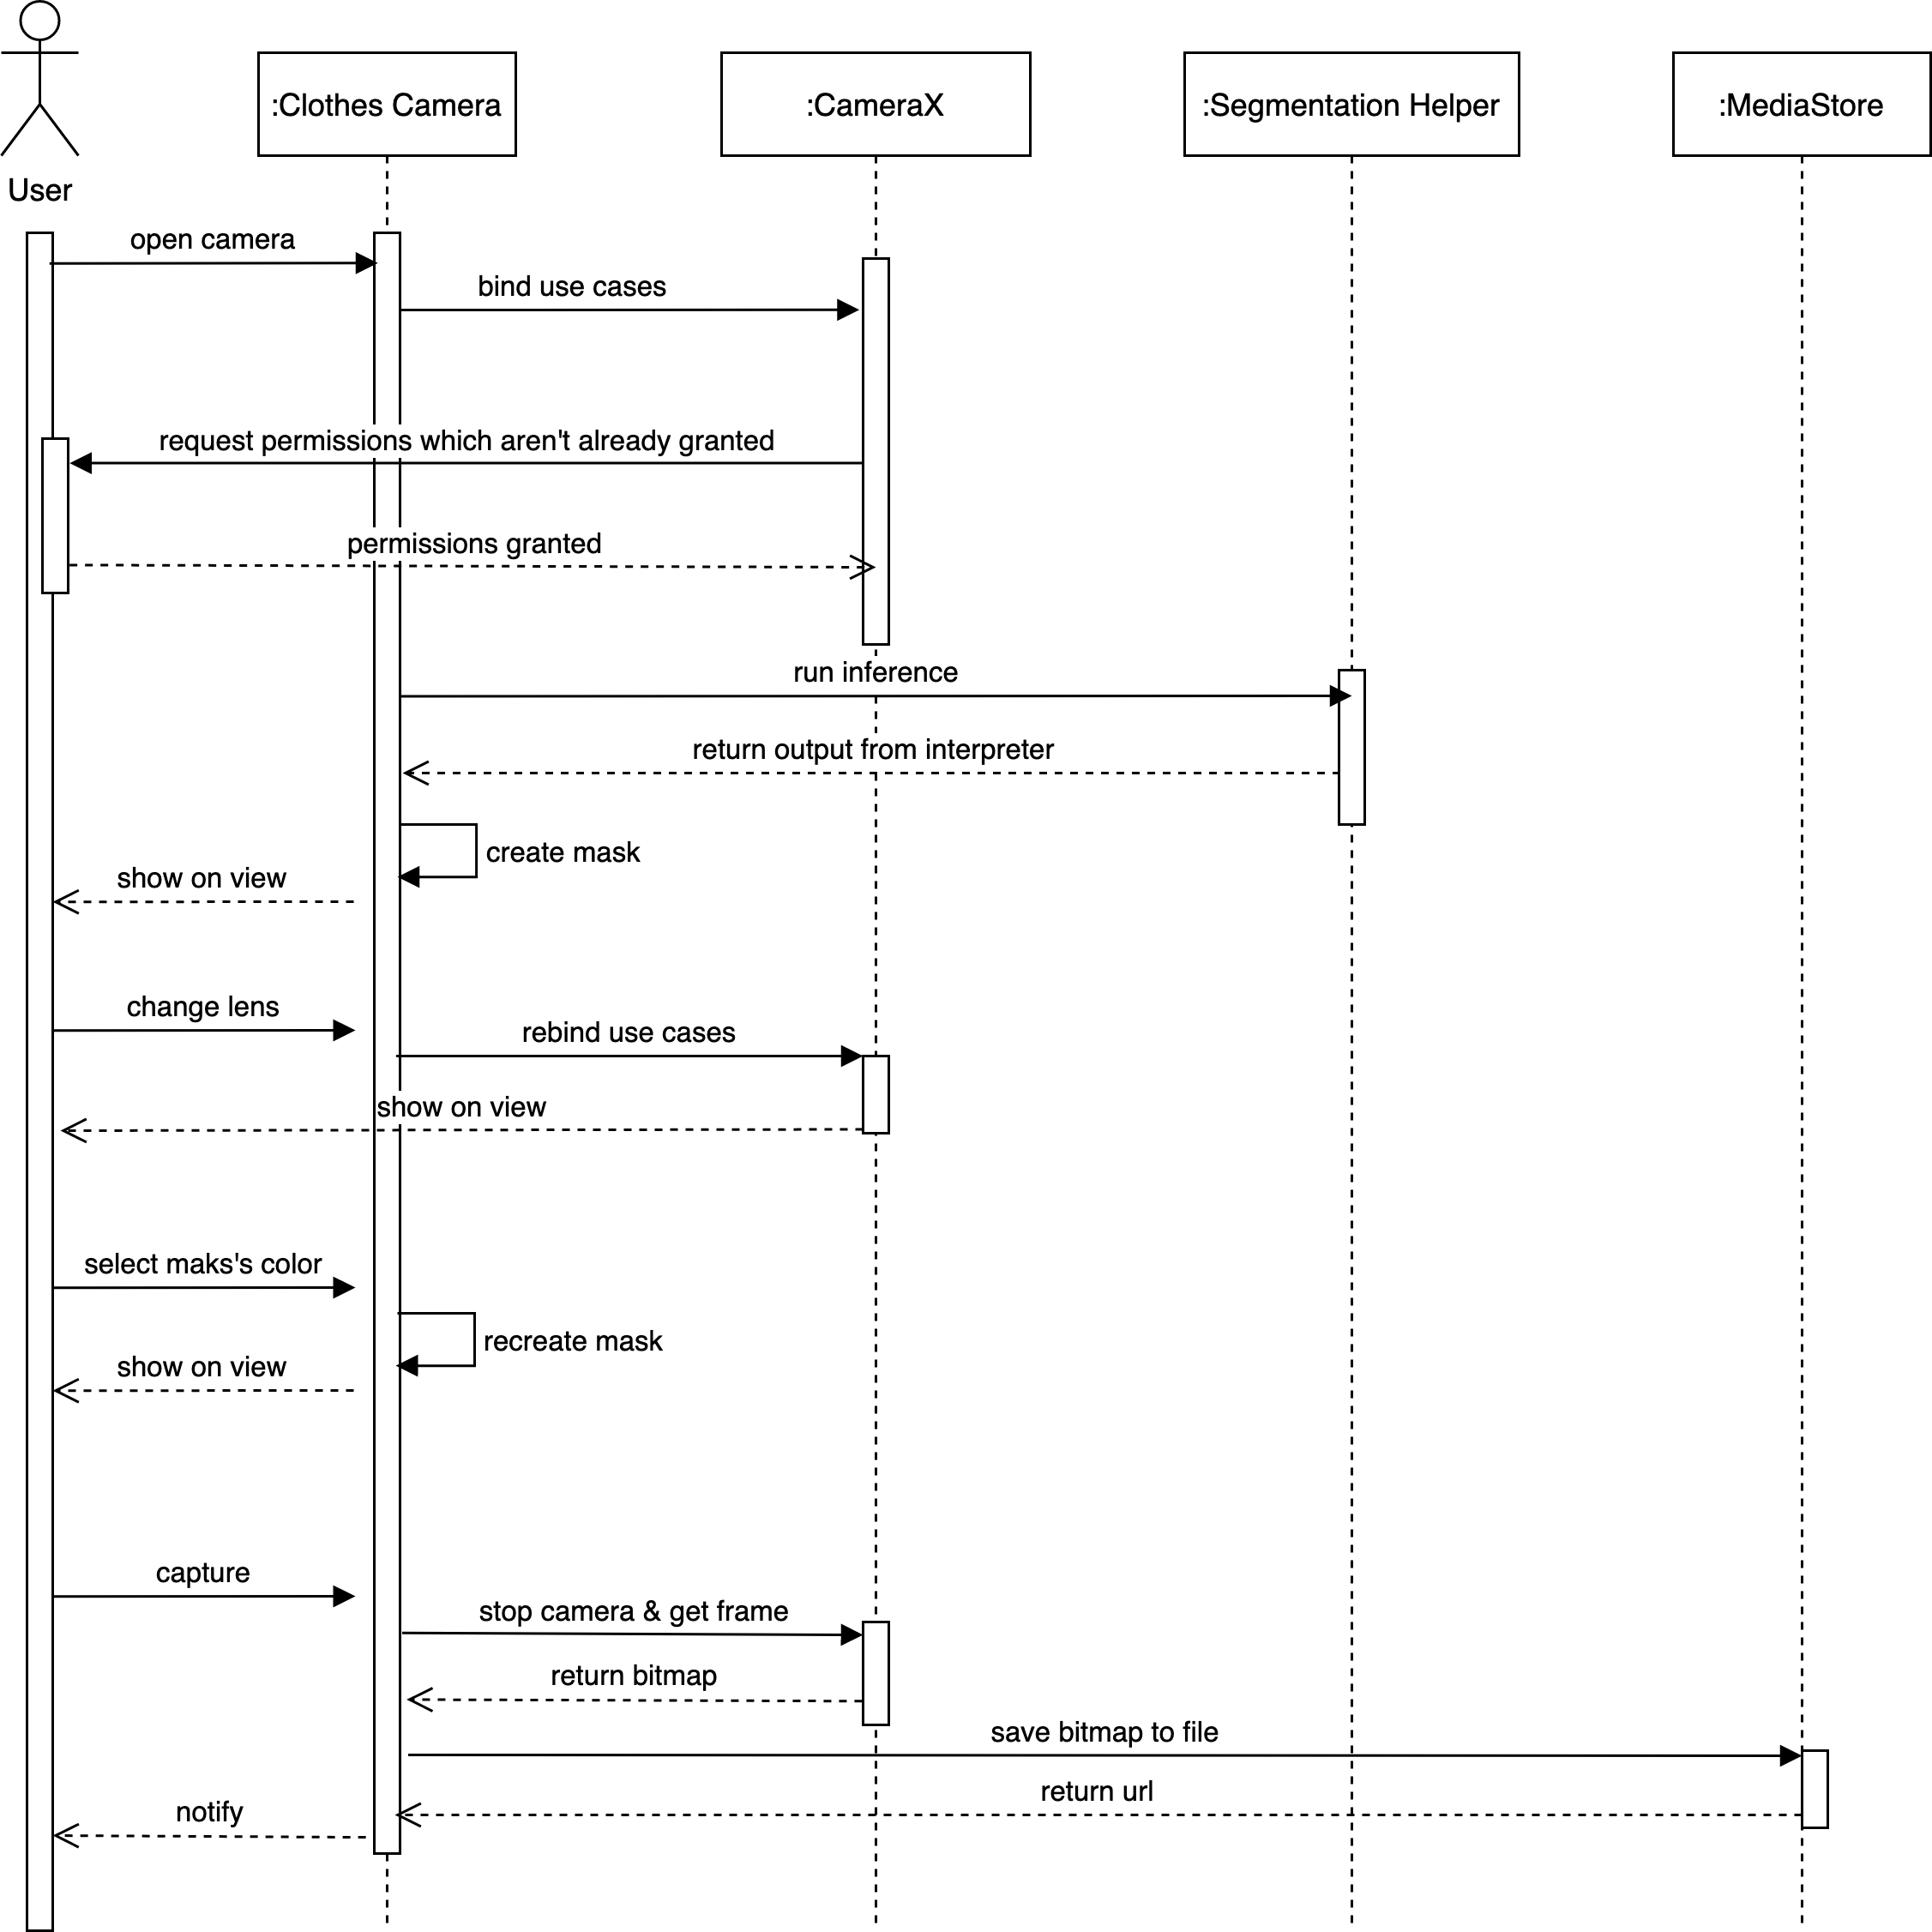
\includegraphics[width=1.0\textwidth]{chapter3/image/clothescamera.png}
    \caption{Sequence diagram for Clothes Camera use case}
    \label{fig:my_label}
\end{figure}

\begin{figure}[H]
    \centering
    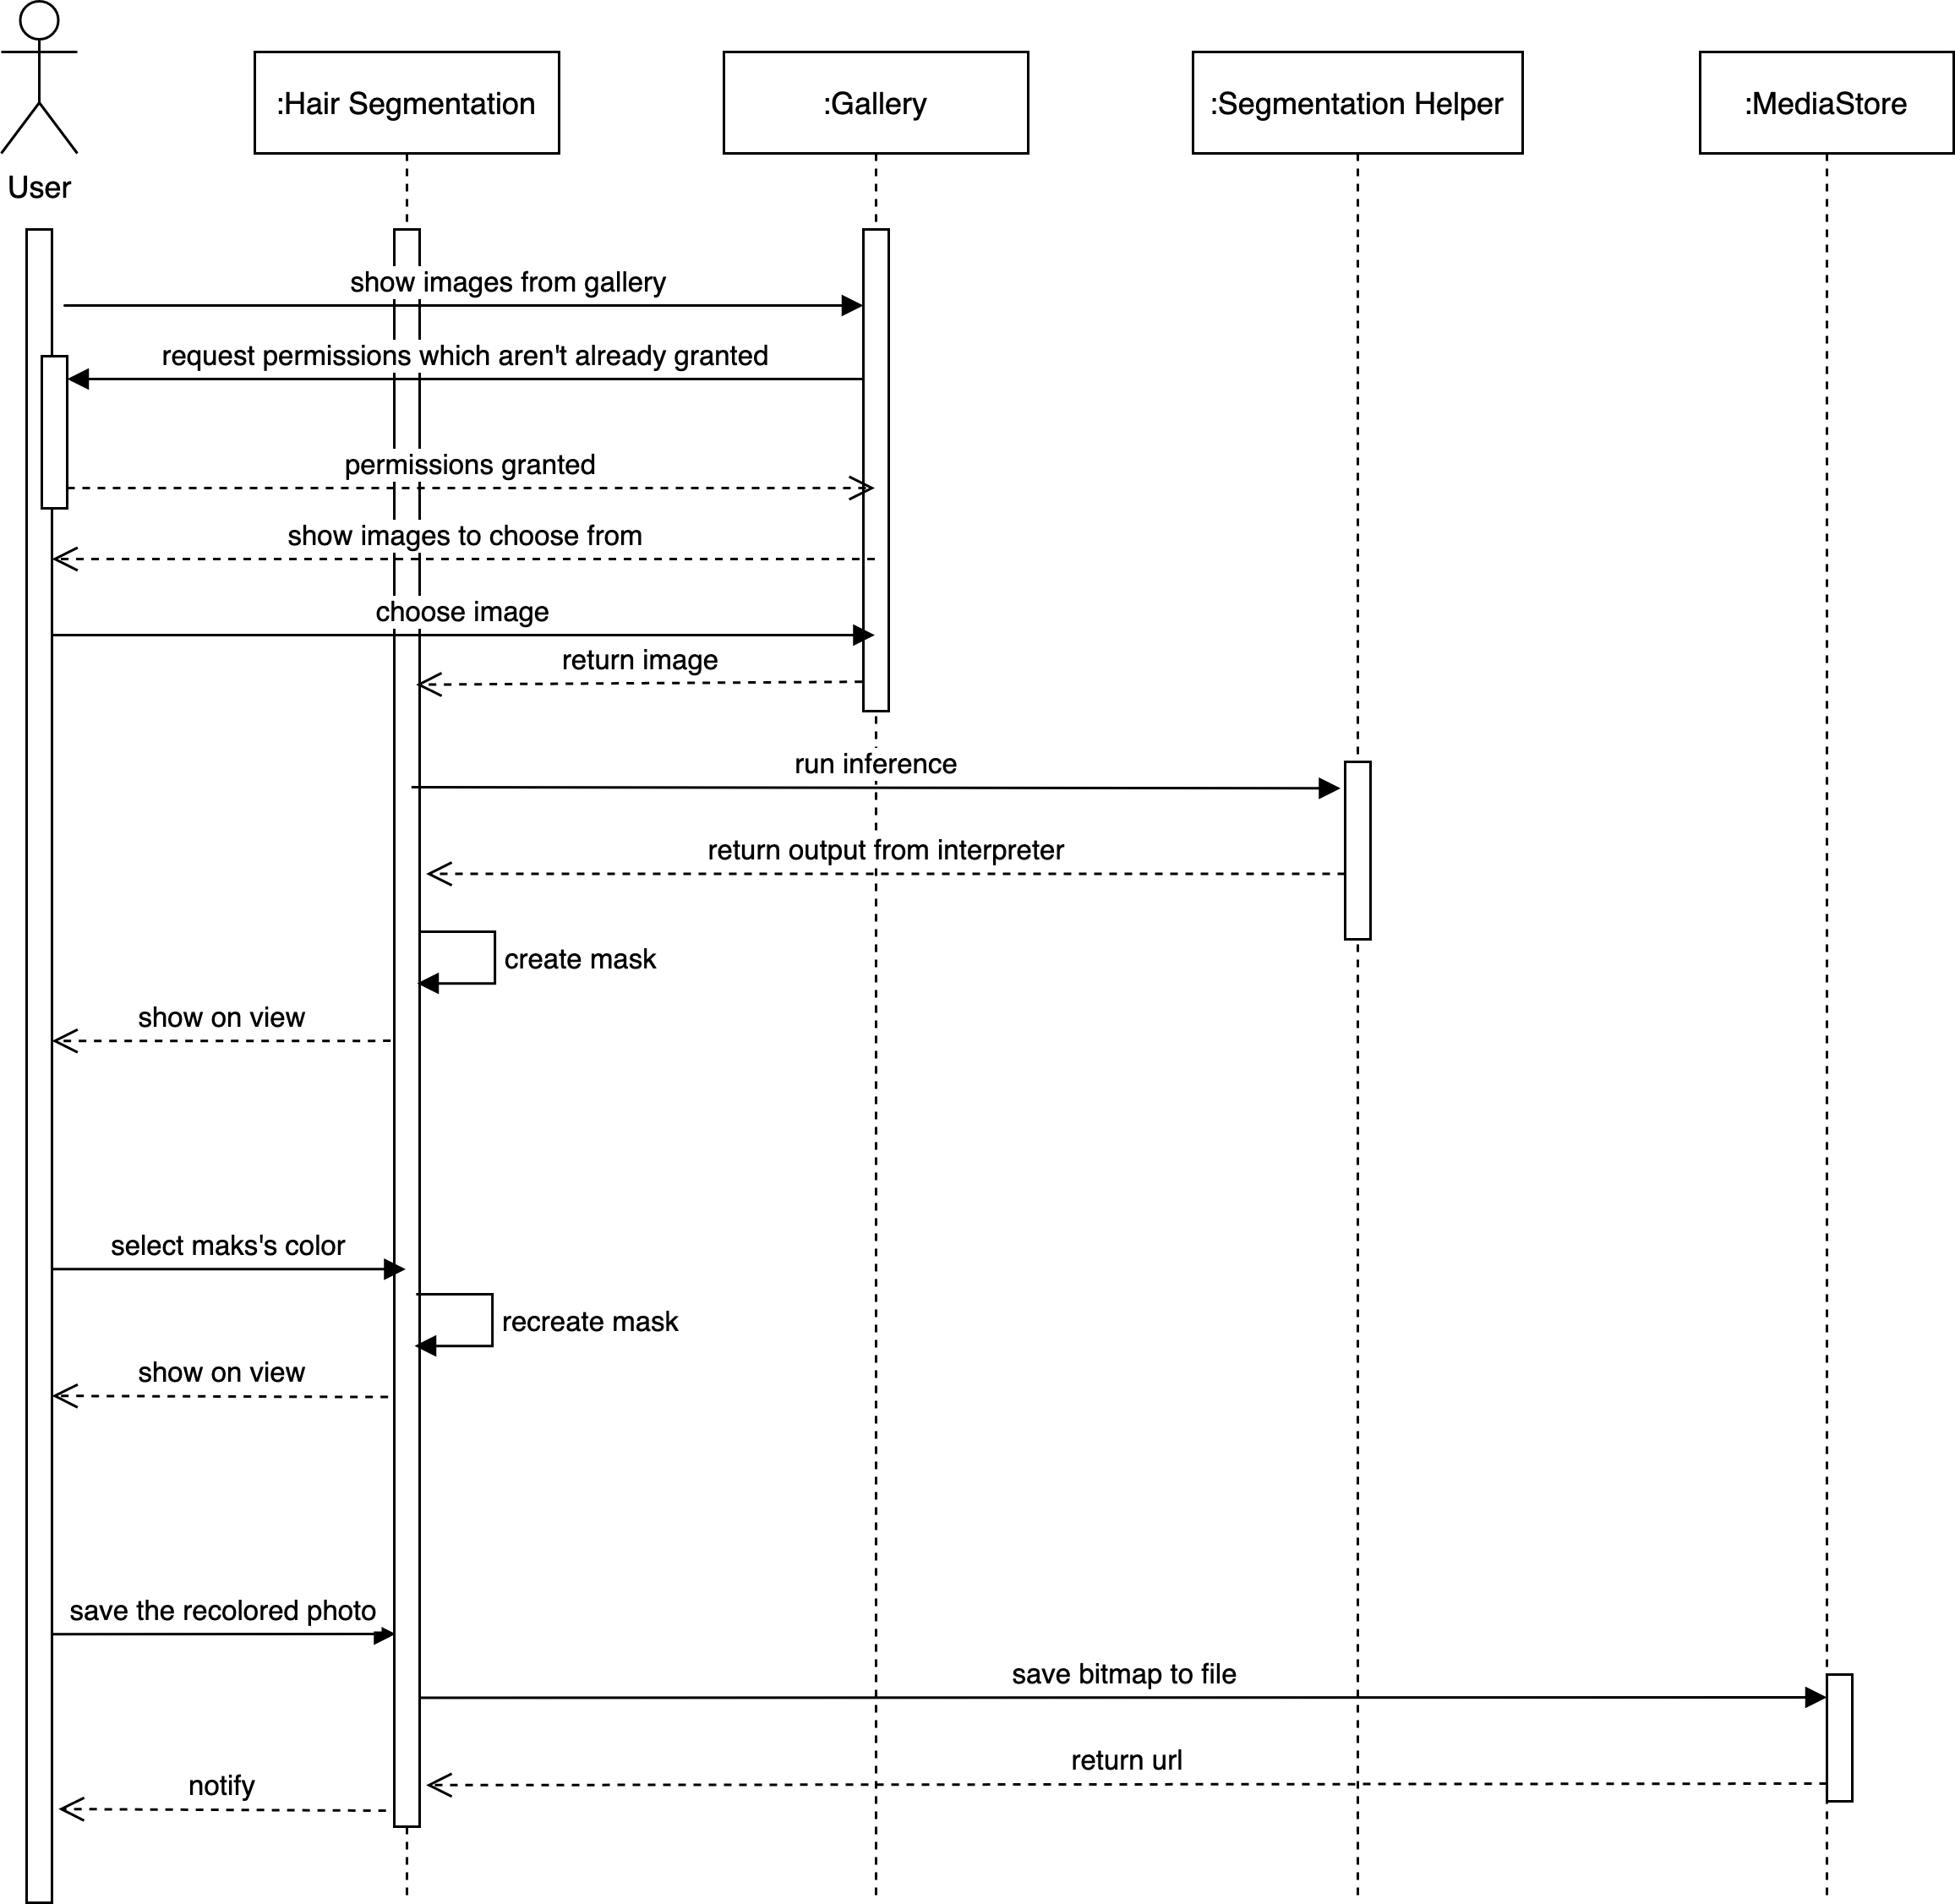
\includegraphics[width=1.0\textwidth]{chapter3/image/hairsegmentation.png}
    \caption{Sequence diagram for Hair Segmentation use case}
    \label{fig:my_label}
\end{figure}
 % 3
\section{Proposed model} \label{sec:model}

Image segmentation models play a vital role in the project and determine the beauty app's latency and user experience. In this section, the proposed CNN is explained, its architecture is about to discuss in more depth. As mentioned previously, as a subset of machine learning, Deep Learning has been showing its accuracy practically in many tasks, such as object detection, object tracking, and object classification. Image segmentation models output a pixel-wise mask of the input image, which is considered as an object segment in the image. Although many DNNs are successful in the image segmentation task in the literature, such as DeepLabV3+ \cite{deeplabv3plus}, PSPNet \cite{pspnet}, they fail to acquire a low latency inference due to their complex architecture in aim to acquire the best accuracy. Considering the requirements, after surveying, I choose U-Net \cite{unet} architecture with MobileNetv2 \cite{mobilenetv2} as a base network for the segmentation tasks. In the following, we dive into the proposed CNN and adaptations to work.
 
 \subsection{MobileNetv2 blackbone}
 MobileNet1 and MobiNetv2 are the first and the second versions in a group of small, low-latency, low-power DNNs named MobileNets. MobileNets is a family of lightweight and general models researched by Google. These models are intended to run with low computational power, such as smartphones, embedded, or IoT devices. Since 2018, when the first version was roll out, there are now three versions with significant improvements after each release. \par
 
 \paragraph{MobiNetv1}
 In MobilNetv1, a key convolution operator called Depth-wise Separable Convolution is first introduced; it takes approximately 70\% less in the number of parameters but only a decrease of 2\% in final accuracy when compared to standard convolution. The basic idea is to replace a full convolutional operator with a factorized one that splits convolution into two separate layers. \par
 
 \begin{figure}[H]
     \centering
     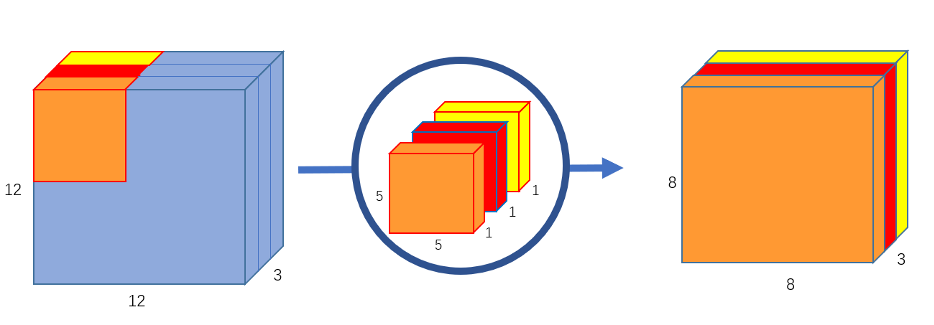
\includegraphics[width=0.9\textwidth]{chapter2/image/mobi1.png}
     \caption{Depthwise convolution, uses 3 kernels (size 5x5) to transform a 12x12x3 image to 8x8x3 image}
     \label{fig:mobi1}
 \end{figure}
 
 \begin{figure}[H]
     \centering
     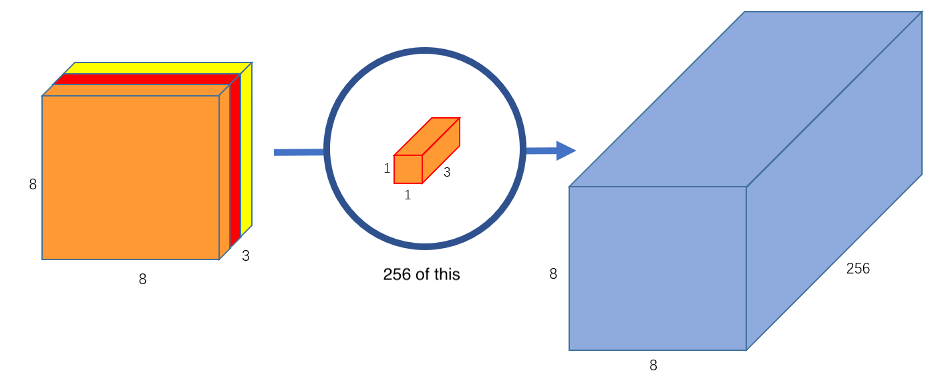
\includegraphics[width=0.9\textwidth]{chapter2/image/mobi2.png}
     \caption{Pointwise convolution, transforms an image of 3 channels (size 8x8x3) to an image of 256 channel (size 8x8x256)}
     \label{fig:mobi2}
 \end{figure}
 
 The entire process can be divvied into two steps: Depthwise convolution and Pointwise convolution. At first, a single-depth convolution is separately applied to each channel of the previous feature map. Take the previous feature map with three channels, illustrated in \textbf{Figure \ref{fig:mobi1}}, Depthwise convolution would consist of three kernels, and each kernel would iterate one channel of the feature map. As the convolutional operations have a single depth, the output has the depth remained the same. Second, N number of Point-wise convolutions are used to combine the outputs of the depth-wise convolution, where N is the desired channel depth of the resulting feature map. In the case of \textbf{Figure \ref{fig:mobi2}}, N is equal to 256. 
 
 \paragraph{MobiNetv2}
 MobileNetV2 is introduced in CVPR 2018, regarded as the next generation of mobile model. It inherits Depthwise Sepratable convolution from MobileNetv1. Although built upon the ideals of MobilNetv1, MobileNetv2 proposes two significant changes to the architecture: linear bottlenecks layers and shortcut connections between the bottlenecks. The basic structure of a bottleneck residual block is shown in \textbf{Figure \ref{fig:mobi2bottleneck}}. \par
 
 \begin{figure}[H]
     \centering
     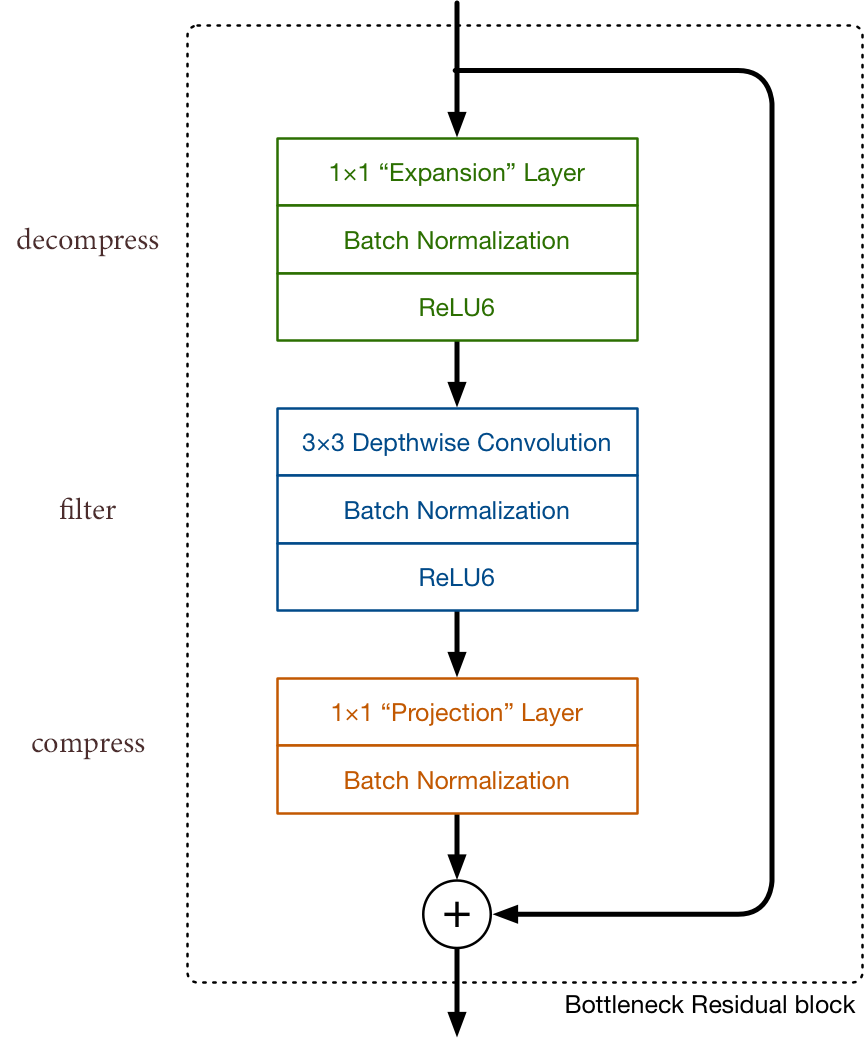
\includegraphics[width=0.6\textwidth]{chapter3/image/block_edited.png}
     \caption{A bottleneck residual block.}
     \label{fig:mobi2bottleneck}
 \end{figure}
There are three convolutional layers in this building block. The first layer is a 1x1 pointwise convolution which is similar to in MobileNetv1.  Its purpose is to expand the number of channels in the data before it goes into the 3x3 depthwise convolution. This expansion layer plays a role as a decompressor that restores the data to its full form. On the other hand, the last convolutional layer, which is also called a bottleneck layer, is a 1x1 pointwise convolution. However, this layer makes the number of channels smaller; in fact, it contrasts to in MobileNetv1 where the pointwise convolution either kept the number of channels the same or doubled them. Its purpose is to projects data with a high number of dimensions (channels) into a tensor with a much lower number of dimensions. In other words, the projection layer compresses the data to make it small again. As a result, the input and the output of the block are low-dimensional tensors, while the filtering step that happens in between is done on a high-dimensional tensor.
 \par
 
 One small change is that the activation function used by MobineNetv2 is ReLU6:
 \begin{equation}
 y = ReLU6(x) = min(max(0, x), 6)
 \end{equation}
 This is like the traditional ReLU as a non-linearity, but it prevents activations from becoming too big. The reason for this is that ReLU6 is more robust than regular ReLU when using low-precision computation. Moreover, the shape of this function is similar to the shape of a sigmoid function. \par
 
 
 I integrate MobinetNetv2 into the overall network excluded the top, which consists of fully-connected layers; otherwise, the image input must be 224x224. MobileNetv2 works as a feature extractor for a second neural network. It is remarked that MobileNetv2 has a good balance between the used resources (memory and FLOPS) and accuracy trade-off. This backbone is far better among other lightweight base networks, such as MnasNet \cite{mnasnet}, SqueezeNet \cite{squeezenet}.
 
 
 \subsection{U-Net architecture} \label{sec:unet}
 This section describes the proposed network entirely. The network is based on the general-purpose U-Net architecture in order to accommodate hair and clothes segmentation tasks. \par
 
 \begin{figure} [H]
     \centering
     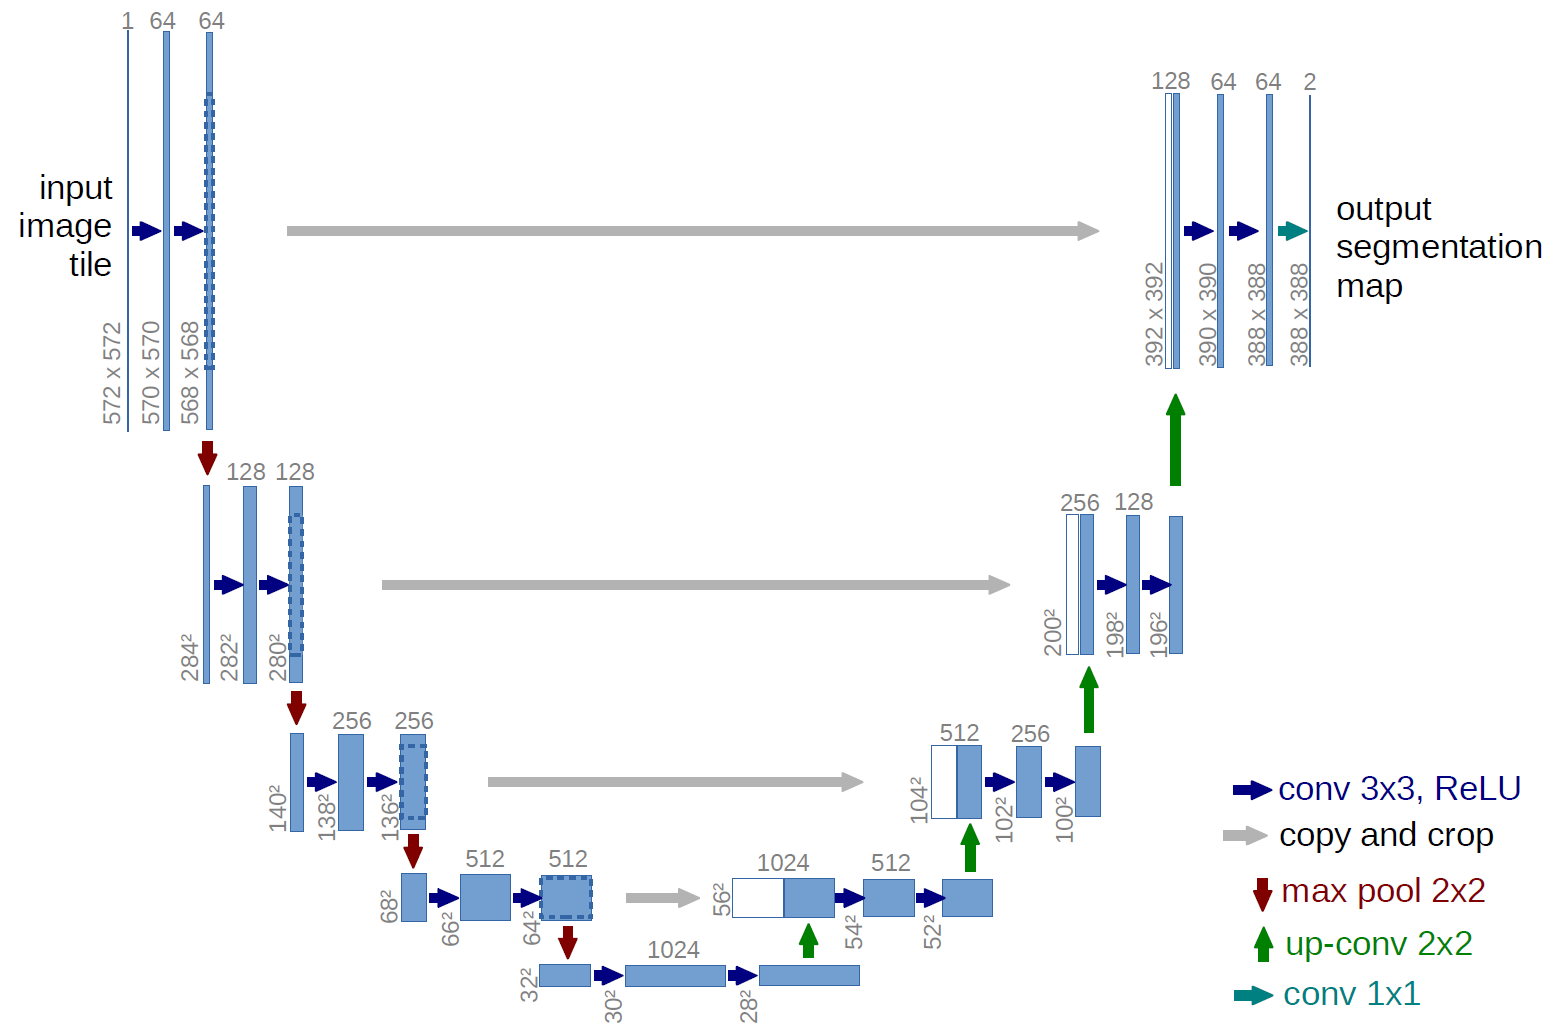
\includegraphics[width=0.7\textwidth]{chapter3/image/u-net.png}
     \caption{Illustration for U-shaped architecture in the origin paper \cite{unet}.}
     \label{fig:unet1}
 \end{figure}
 
 U-Net is an autoencoder type network architecture introduced in \cite{unet} for semantic segmentation of biomedical images in 2015. However, U-Net achieves high accuracy in other segmentation tasks as well. It introduces skip-connections to the autoencoder architecture to improve resolving and propagating higher-level features in the decoder block.
As a consequence, the decoder can access information from the encoder, such as edges, corners and angles in the original images. Many semantic segmentation networks utilize this ideal where information from the encoder is passed to the decoder via long skip-connections to preserve higher-level information found at higher resolutions in the encoder. \par

\vspace{5mm}

 \begin{figure} [H]
     \centering
     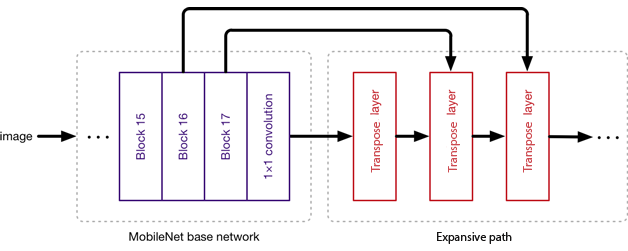
\includegraphics[width=0.9\textwidth]{chapter3/image/architec.png}
     \caption{UNet architecture with the MobileNetv2 base model.}
     \label{fig:unet2}
 \end{figure}
 
 While \textbf{Figure \ref{fig:unet1}} depicts the origin U-Net architecture in view of layers, \textbf{Figure \ref{fig:unet2}} shows the adapted network in view of components. More specifically, the contracting path replicates the architecture of MobileNetv2 with 17 blocks in total. On the other hand, the expansive path consists of an upsampling of feature maps followed by a 2x2 convolution that halves the number of feature channels. The upsampling method is transposed convolutions. The number of max-pooling layers 
 equal to the number of transposed convolutions and equals five. Generally, the proposed network has the same architecture as the original version; however, I made slight modifications.
 The first adaptation I made is that batch normalization is only used in the contracting path of the network. It changes results from preliminary experiments and increases the speed of the network without decreasing the accuracy. The second adaptation lies at the two last layers, where the last convolution has a kernel size of one and is followed by a softmax activation. As a result, the network would output a final probability map, which represents the desired mask. Following that, the loss is calculated as a binary cross-entropy function on a pixel-wise basis.
 \par % 3


\section{App Development}  \label{androidapp}
In previous section, DNN for hair and clothes segmentation has been reviewed. In this section, proposed solution to the task of intergrating the model into the Android app is demonstrated. Consequently, the implementation of an Android app is rather easy once you have a proper design and well-defined solutions. 
\subsection{Pipeline}
One of the most important use cases of common beauty or augmented reality applications is real-time camera visuality. In case of the thesis, the beauty app has two instance of these use cases: \emph{Hair Camera} and \emph{Clothes Camera}. Indeed, they are addressed as the most intricate work in the app. To clear it up, I proposed a pipeline used for both the two use cases, however the proposed pipeline is so general that can be reused in other applications.  

\vspace{3mm}
\begin{figure} [H]
    \centering
    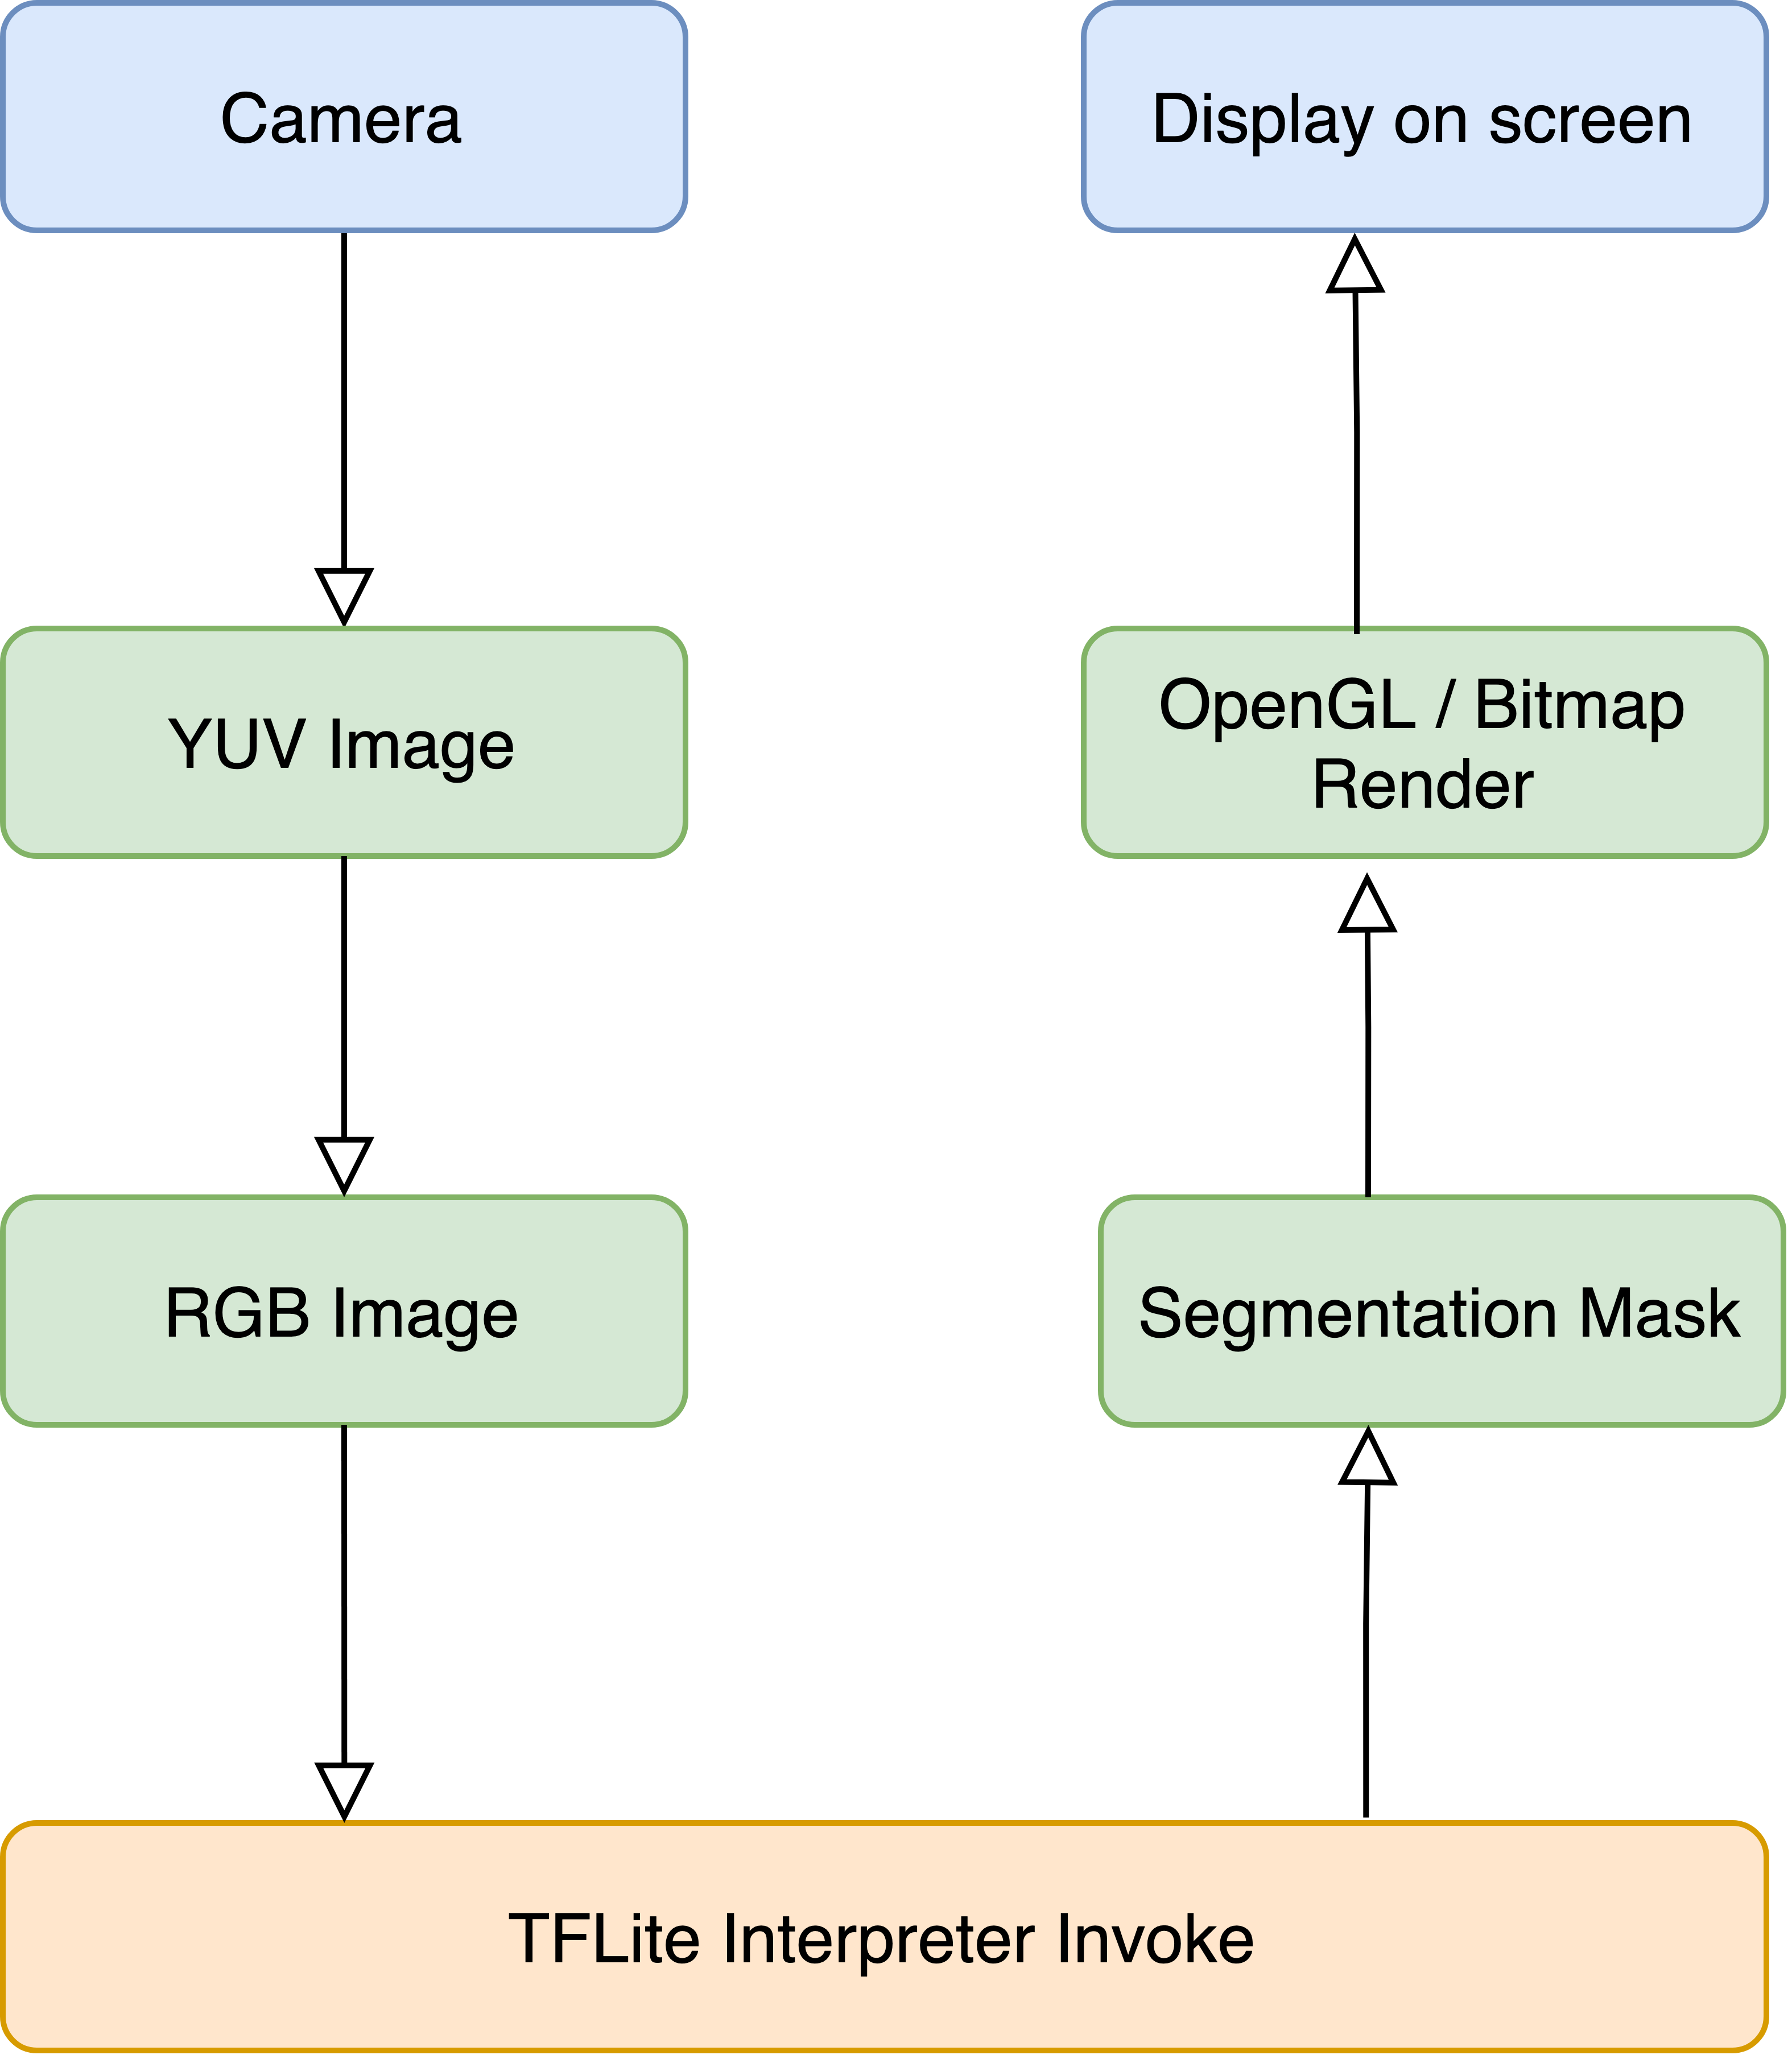
\includegraphics[width=0.6\textwidth]{chapter3/image/apppipeline.png}
    \caption{Pipeline for camera use case}
    \label{fig:my_label}
\end{figure}
 
The pipeline starts with receiving data from hardware, here is the camera lens. CameraX library, which is mention in \textbf{section \ref{sec:camerax}}, supports entire this work.  However, each camera framework outputs image under a different format. For example, if app uses CameraX or Camera2 API, output images are in YUV\_420\_888 format. If app uses Camera API, output images are in NV21 format. After that, the image is converted to a RGB image and represented as byte buffer in order to feed to the model. Subsequently, the TFLite interpreter, which is situated in middle, receives input buffer and outputs the result buffer of the model. The buffer is then preprocessed before being rendered. Finally, the mask is displayed on screen, as a result, the camera view is overlaid with the mask.

 
\subsection{On-device inference}

Making an inference involves taking single or multiple inputs (images, text, video) and pushing them through the many layers of the network. In matters of making on-device predictions, it is vital to have a general understanding of hardware types where the model runs. Almost all smartphones have both CPUs and GPUs. In Android, there are even a few libraries that work with these hardware platforms in order to supply accelerators for deep learning.  \par

Android Neural Networks API (NNAPI) is one of them, which is available for Android 8.1 and above. NNAPI is a machine learning library that supports a wide variety of chipsets, including Snapdragon. There are three options for hardware accelerators, namely GPU, NNAPI, and CPU. Technically, NNAPI is an Android C API designed for executing computationally intensive operations for machine learning on Android devices. NNAPI runtime is a shared library that situated between an app and backend drives, enables NNAPI to run on multiple mobile platforms (Snapdragon, AMD...) \par
 \begin{figure} [H]
     \centering
     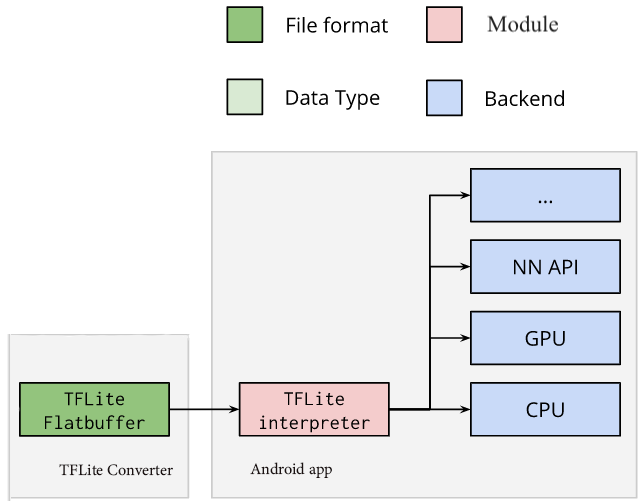
\includegraphics[width=0.7\textwidth]{chapter3/image/client pipleline_edited.png}
     \caption{Workflow of TFLite library for Android}
     \label{fig:my_label}
 \end{figure}
Built upon this, TFLite Interpreter in Android develops both NNAPI delegate and GPU delegate. The GPU delegate is optimized to run 32-bit and 16-bit float-based models where a GPU is available. Although the GPU delegate is well-run and supports more operating systems, I find the NNAPI delegate more effective and battery saving. The following is the code used for preparing input data and run inference with TFLite:\par 
\vspace{5mm}

\begin{lstlisting}[ caption=NNAPI Inference implementation]
// Image pre-processing before feeding into the DNN
private val tfImageProcessor by lazy {
    val cropSize = minOf(bitmapBuffer.width, bitmapBuffer.height)
    ImageProcessor.Builder()
        .add(ResizeWithCropOrPadOp(cropSize, cropSize))
        .add(ResizeOp(
            tfInputSize.height, tfInputSize.width,
            ResizeOp.ResizeMethod.BILINEAR))
        .add(Rot90Op(-imageRotationDegrees / 90))
        .add(NormalizeOp(127.5f, 127.5f))
        .build()
}

// Initialize interpreter with GPU delegate
private val tflite by lazy {
    Interpreter(
        FileUtil.loadMappedFile(this, MODEL_PATH),
        Interpreter.Options().addDelegate(NnApiDelegate())
    )
}

val output =  tflite.run(tfImageProcessor.process(input))
\end{lstlisting}
 
 
 
 
 
 
 
\subsection{Rendering masks}
After semantic information is obtained from the interpreter, segmentation maps are generated. In order to format and display them, two methods of rendering are proposed, namely Bitmap and OpenGL.

\subsubsection{Bitmap}
A bitmap is simply a rectangle of pixels. Each pixel can be set to a given color but exactly what color depends on the type of the pixel. A so-called type of pixels is \emph{ARGB\_8888} where a pixel has four channels (Alpha, Red, Green, Blue) and allocates each eight bits of storage.\par

Bitmap is the first rendering method applied to the app because its well-support in Android API. In fact, Bitmap is a popular 2D graphics class, and Android allows you to use the \emph{Bitmap} class for working with bitmaps. It extends from \emph{Drawable} class which is a general and abstract class for something that can be drawn.  \par


\begin{lstlisting}[caption=Bitmap rendering implementation]
val mask = Bitmap.createScaledBitmap(output, screen.width, screen.height)

overlay.setImageBitmap(
    mask
)
\end{lstlisting}

It would be effective if you do not modify bitmaps too often, because every time you change the content of a bitmap, it is uploaded again as a GPU texture the next time you draw it. As a result, there would have a delay. \par

\subsubsection{OpenGL ES}
OpenGL is a well-used open-source graphic library for rendering 2D and 3D vector graphics on almost all platforms. Android OS is not an exception; it uses a subset of OpenGL’s API called OpenGL for Embedded System (OpenGL ES). OpenGL ES is cross-platform, albeit closed-source. In Android, OpenGL ES is loaded to NDK as a shared library, and SDK wraps it up for ease of implementation.
\par

\begin{figure} [H]
    \centering
    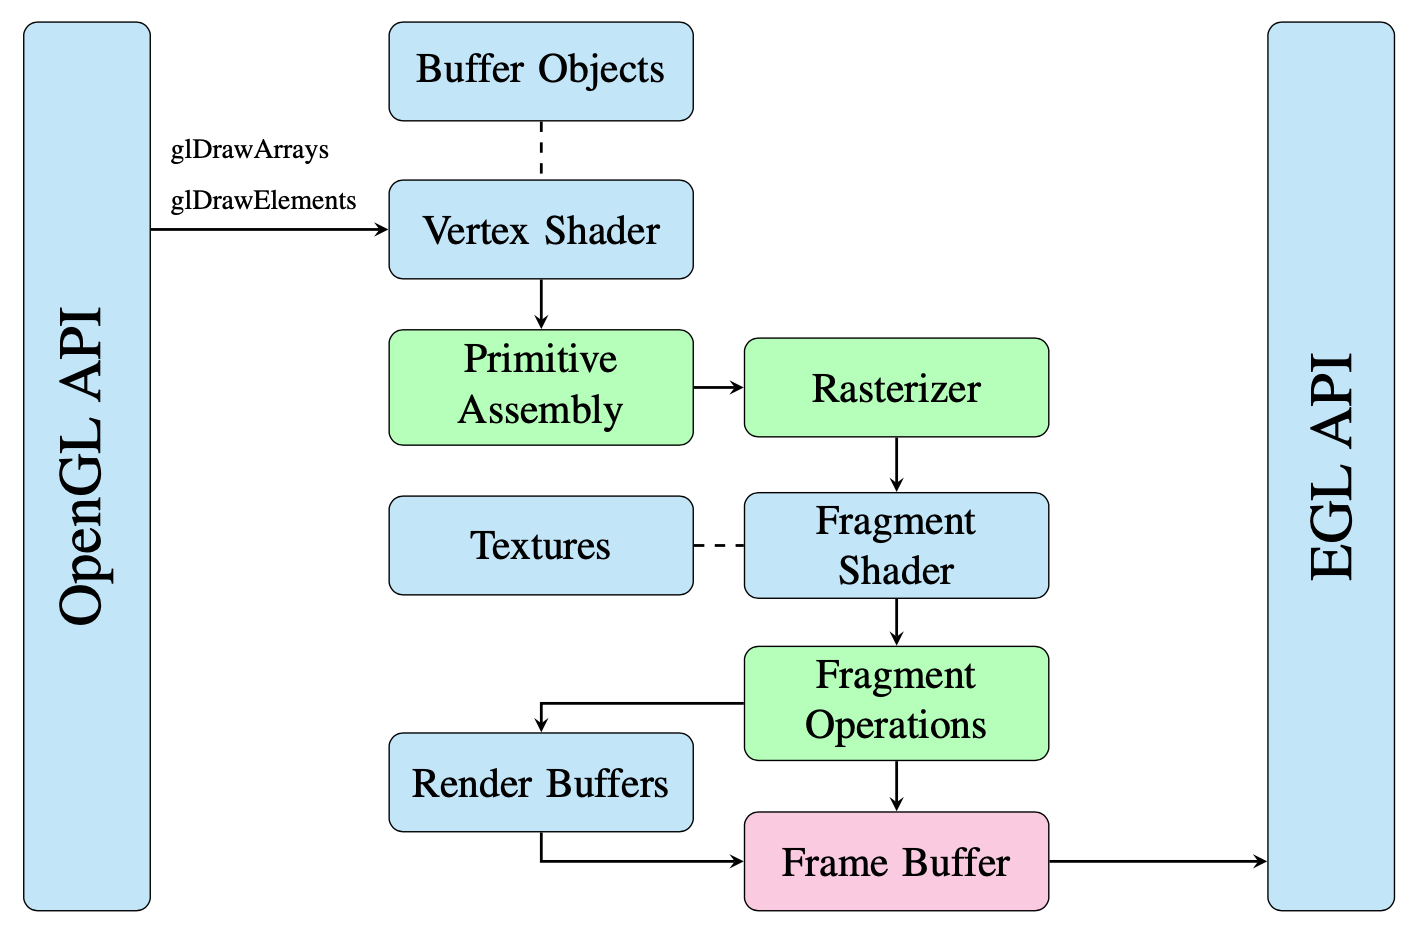
\includegraphics[width=0.7\textwidth]{chapter3/image/openglpipeline.png}
    \caption{OpenGL ES 2.x pipeline. Blue node: You have to set, Green node: You do not have any control, Magenta node: Optional. Source: \cite{openglpipeline}.}
    \label{fig:coordinates}
\end{figure}

The first step in the rendering process is sending the vertices and the texture positions along with the textures, as shown in \textbf{Figure \ref{fig:coordinates}}. To do so, the points that were passed to the renderer first combined into a 1-dimensional array of (x,y,z) values, then uploaded to the vertex shader along with the corresponding texture coordinates of the segmentation mask. These values fall into the range of [−1, 1] in the GLES coordinates, where the point (0, 0) being the middle of the screen. However, the texture coordinates are ranged from [0, 1] where point (0, 0) being the bottom left corner. After the coordinate is uploaded to the vertex shader, the textures are sent to the fragment shader. In the implementation, it was found that it is more efficient to load the whole mask's texture before starting the drawing loop.\par



%We send two different textures to the shader. The segmentation mask which consists of one channel and the color image of the original scene to perform the inpainting in the fragment shader. These textures are sent after the segmentation mask is generated and the hit test is performed by using GLES interface function glTexImage2D. \par

 % 3
